\chapter{Introduzione}
\label{chap:1}



\section{Contestualizzazione e Motivazioni}
\label{sec:Contestualizzazione}

\subsection{Evoluzione delle applicazioni web}
Inizialmente le applicazioni web erano costituite da semplici pagine statiche contenenti testo e immagini.
Col passare degli anni, grazie all'adozione di JavaScript e di librerie e framework correlati, hanno progressivamente acquisito un carattere più dinamico, con l'introduzione di livelli crescenti di interattività. 
Un cambiamento significativo in tal senso, è avvenuto con l'avvento delle Single Page Application (SPA) e di AJAX.
Tale combinazione, ha infatti introdotto un nuovo paradigma di sviluppo, in cui l'intera appplicazione viene caricata una sola volta e le successive interazioni con l'utente avvengono grazie al caricamento dinamico di contenuti e dati provenienti da un web server, eliminando così l'attesa nel caricamento di una nuova pagina e favorendo l'esperienza d'uso.
\\Parallelamente, la complessità delle funzionalità offerte è cresciuta in modo esponenziale, spaziando da applicazioni di grafica 3D, a simulatori, ad applicazioni di modifica di documenti, immagini e video.
Oggi, è sempre più comune incontrare siti web in grado di gestire complesse operazioni in tempi rapidi, assicurando così quell'interattività alla quale ormai siamo abituati. 
Tuttavia questo progresso è stato accompagnato da un aumento del numero di richieste effettuate in rete e dall'utilizzo intensivo di risorse computazionali, sia lato cliente, che lato servitore.
\begin{figure}
        \begin{center}
                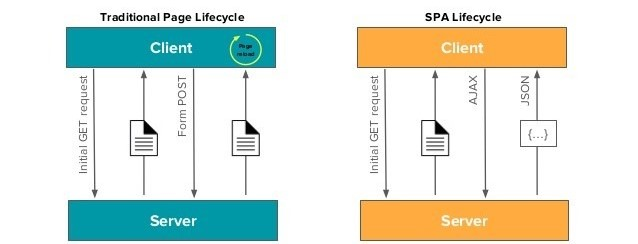
\includegraphics[width=0.61\columnwidth]{images/spa.jpg}
        \end{center}
        \caption{Differenza nel tipo di richieste tra SPA e MPA.}
        \label{fig:spa}
\end{figure}
        
\subsection{Importanza dell'ottimizzazione}

\section{Obiettivi}
\label{sec:Obiettivi}
Si è scelto di svil

\subsection{Analisi Comparativa delle Tecnologie}

\subsection{Valutazione dell'Impatto di Wasm}




\section{Trend di evoluzione del web}
\label{sec:Trend}
\subsection{Paradigmi di Sviluppo Moderni}

\subsection{Esperienze Utente Migliorate ?}



\section{Struttura della tesi}
\label{sec:struttura}

This is a reference to a chapter \ref{chap:1}. This is a reference to a figure \ref{fig:doge}. This is a reference to some code \ref{lst:hello}. This is a citation \cite{famous:paper}.

\lstinputlisting[label=lst:hello, firstline=2, lastline=4, caption={I directly included a portion of a file}]{code/hello.py}

\begin{lstlisting}[language=Java, label=lst:java, caption={Some code in another language than the default one}]
public void prepare(AClass foo) {
        AnotherClass bar = new AnotherClass(foo)
}
\end{lstlisting}


\begin{figure}
\begin{center}

\includegraphics[width=0.3\columnwidth]{images/doge.png}
\end{center}
\caption{This is not a figure. It's a caption.}
\label{fig:doge}
\end{figure}
